%----------------------------------------------------------------------------
\chapter{Használt technológiák}
\label{chapt:birdmap-technologies}
%----------------------------------------------------------------------------
Ezzel a fejezettel az a célom, hogy ismertessem a fejlesztés során, illetve az alkalmazásom által használt technológiákat,
hogy a következő fejezetekben alapozni tudjak ezeknek az ismeretére.

%----------------------------------------------------------------------------
\section{A fejlesztési folyamat technológiái}
%----------------------------------------------------------------------------
Ebben a szakaszban azokat az eszközöket, alkalmazásokat és fejlesztőkörnyezeteket mutatom be, melyeket a fejlesztés során, a fejlesztéshez használtam. 

%----------------------------------------------------------------------------
\subsection{Git}
%----------------------------------------------------------------------------
A Git \cite{git} egy verziókezelő rendszer. Használatával a felhasználó le tudja menteni egy adott fájlrendszerben található fájlok állapotát.
Megkönnyíti az egy projekten dolgozó programozók közötti kooperációt. Manapság lassan elképzelhetetlen a fejlesztés valamilyen verziókezelő használata nélkül.

%----------------------------------------------------------------------------
\subsection{Trello}
%----------------------------------------------------------------------------
A Trello \cite{trello} egy webes projektmenedszment alkalmazás. 
Azért használtam a fejlesztés során, mert szerettem volna egy helyet, ami tükrözi a fejlesztés állapotát, ahova le tudom írni az alkalmazással kapcsolatos ötleteimet.
Különböző listákban tároltam a fejlesztésre váró és a kész feladatokat szerver, kliens és egyéb szerint.

\begin{figure}[!ht]
    \centering
    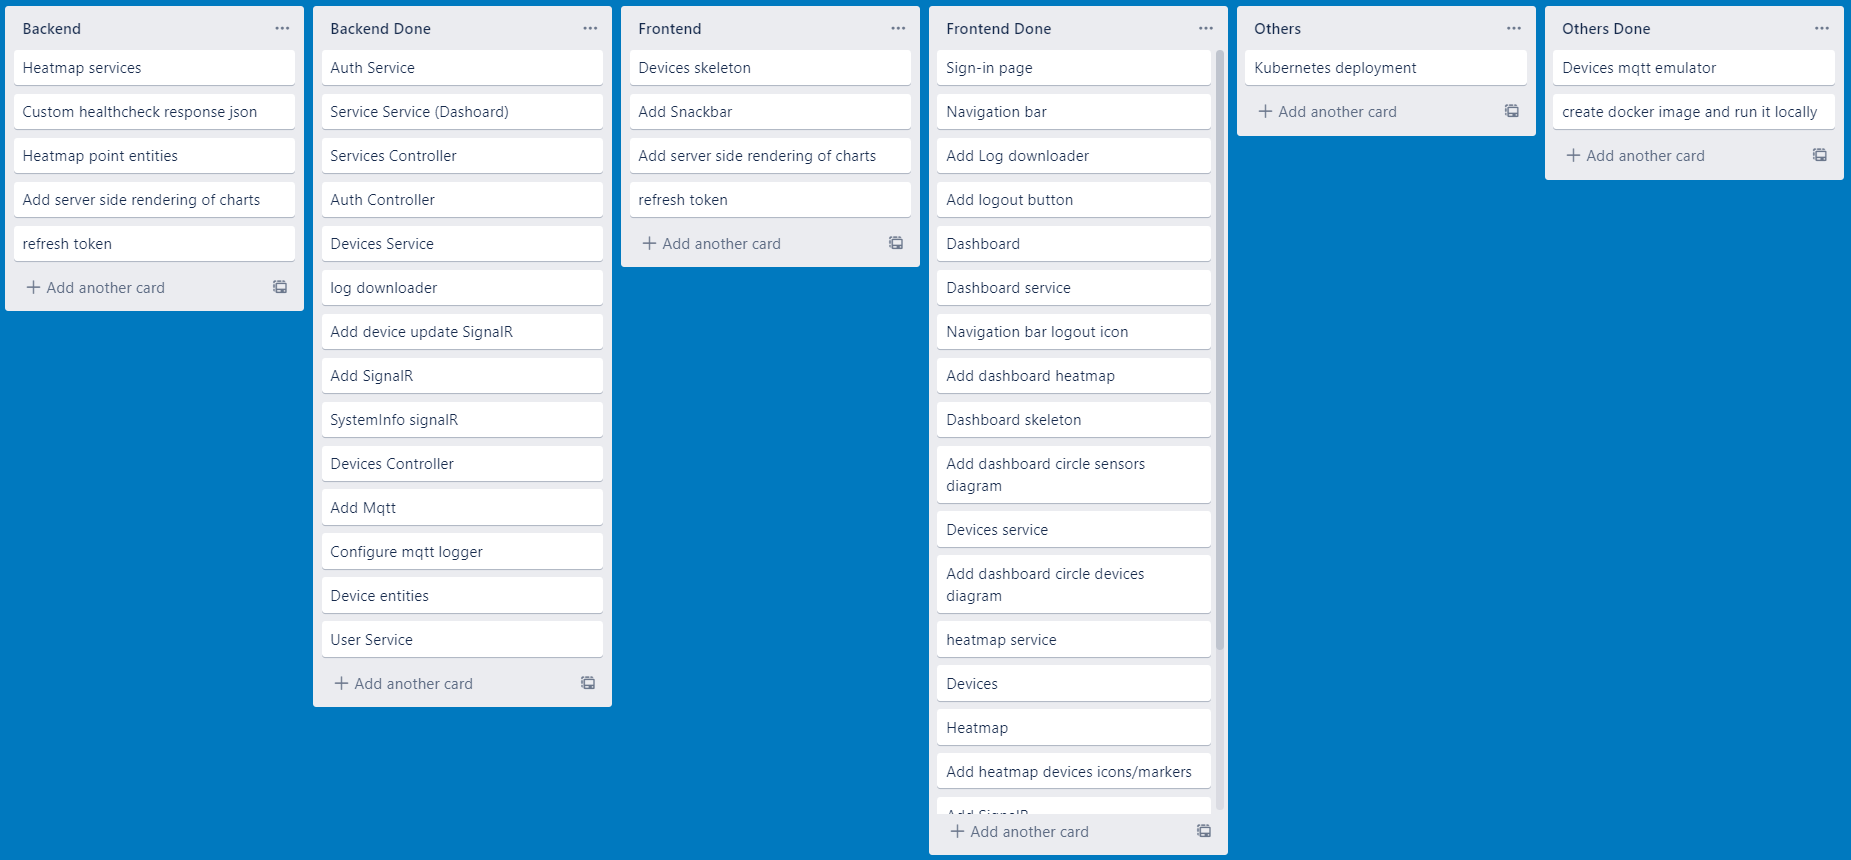
\includegraphics[width=150mm, keepaspectratio]{figures/trello-3.png}
    \caption{Egy példa állapot a Trello felületére a fejlesztés során}
    \label{fig:trello}
\end{figure}

%----------------------------------------------------------------------------
\subsection{Visual Studio}
%----------------------------------------------------------------------------
A Visual Studio \cite{vs} a Microsoft fejlesztőkörnyezete. Jól alkalmazható a .NET keretrendszer technológiáival, ezért ezt használtam a szerveroldal fejlesztése során.

%----------------------------------------------------------------------------
\subsection{Visual Studio Code}
%----------------------------------------------------------------------------
Egy másik Microsoft termék, viszont a fentivel ellentétben a Visual Studio Code \cite{vs-code} inkább szövegszerkeztő, mint fejlesztőkörnyezet.
Ennek köszönhetően jelentősen gyorsabb és egyszerűbb a használata. Különféle bővítmények használatával nagyon jó program nyelv támogatottságot lehet elérni.
Többek között ezen okok miatt preferáltam a kliensoldal fejlesztésére. 

%----------------------------------------------------------------------------
\section{Backend technológiák}
%----------------------------------------------------------------------------
Ebben a szakaszban a szerveroldal megvalósítására használt .NET technológiákat mutatom be. A választásom több ok miatt esett a .NET keretrendszer használatára.

Egyrészt úgy gondoltam, hogy az alkalmazásom fajsúlyosabb részét inkább a kliensoldal fogja képezni ezért, hogy arra több energiát tudjak fordítani, valami olyat választottam,
amivel már foglalkoztam korábban, amivel gyorsabban és rutinosabban megy a fejlesztés.

Másrészt nemrég jelent meg a .NET új 5-ös verziója, melynek használatával jelentős teljesítmény javulást ígértek több területen is, és úgy gondoltam, hogy ez a projekt tökéletes lenne
ennek próbatételére.

Mindemellett a .NET teljesen platformüggetlen, mely az egyik legfontosabb követelmény volt az alkalmazással szemben.

%----------------------------------------------------------------------------
\subsection{ASP.NET Core}
%----------------------------------------------------------------------------
Az ASP.NET Core a .NET család ingyenes, nyílt forráskódú webes keretrendszere. Gyors és moduláris fejlesztést tesz lehetővé, 
mely főként a csomagkezelő rendszerének, a NuGet-nek \cite{nuget} köszönhető.
Használatána egyik előnye, hogy ugyan az a C\# kód tud futni a szerver éa a kliens oldalon, de támogat más kliens oldali keretrendszereket is, mint például az Angular-t, a Vue.js-t
vagy a React.js-t.

%----------------------------------------------------------------------------
\subsection{Entity Framework Core}
%----------------------------------------------------------------------------
Az Entity Framework Core (röviden EF Core) egy objektum-relációs leképező keretrendszer a .NET-hez. Az adatbázissal való kommunikációt könnyítését szolgálja. 
Használatával C\#-ban lehet adatbázis lekérdezéseket írni a LINQ (Language-Integrated Query) szoftvercsomag segítségével.

%----------------------------------------------------------------------------
\subsection{JSON Web Token}
%----------------------------------------------------------------------------
Az autorizációt többféleképpen meg lehet oldani egy alkalmazás szempontjából. Az egyik ilyen megoldás a JSON Web Token-ek (röviden JWT) \cite{jwt} használata,
ami nem más mint egy szabvány, mely módszert ad a felek közötti információ biztonságos továbbítására JSON objektumokkal.
Ezen objektumok adatokat tárolhatnak a felhasználóról például a neve vagy a szerepe, melyek segítségével a szerver eldöntheti, 
hogy van-e jogosultsága hívni az adott végpontot.

A Microsoft-nak van egy beépített szoftvercsomagja, mellyel ilyen tokeneket lehet készíteni és validálni.
A szerveroldal jogosultság kezelését ezzel a csomaggal oldottam meg.

%----------------------------------------------------------------------------
\subsection{SignalR}
%----------------------------------------------------------------------------
A SignalR \cite{signalr} egy .NET szoftvercsomag, mely lehetővé teszi a szerveroldal számára a kliensekkel való aszinkron kommunikációt.
A szerver valós időben tud értesítéseket küldeni a kliensek számára, amelyek feliratkoztak az ilyen eseményekre.

%----------------------------------------------------------------------------
\subsection{MQTT.NET}
%----------------------------------------------------------------------------
Az MQTT.NET \cite{mqttnet-github} is egy .NET szoftvercsomag, mely a Birbnetes által is használt, a \ref{subsect:mqtt}-es alfejezetben bemutatott MQTT kommunikáció C\# nyelvű megvalósítását szolgálja.

%----------------------------------------------------------------------------
\subsection{NLog}
%----------------------------------------------------------------------------
A szerveroldali naplózás megvalósítására több szoftvercsomag is létezik. Az NLog \cite{nlog}-ot választottam, egyrészt mert egyszerű a használata,
másrészt mert már korábban használtam. Konfigurációs fájljában meg lehet adni a naplózott események célját, mely lehet akár fájl vagy konzol is.
Meg lehet még adni az események elrendezését, hogy azok milyen formában kerüljenek a célokba, milyen plusz információt tartalmazzanak.

%----------------------------------------------------------------------------
\section{Frontend technológiák}
%----------------------------------------------------------------------------
Ebben a szakaszban a kliensoldalon használt technológiákat mutatom be. 
Választásomnál fő motiváció az volt, hogy szerettem volna valami újat kipróbálni, aminek nincs köze a .NET keretrendszerhez.

%----------------------------------------------------------------------------
\subsection{React.js}
%----------------------------------------------------------------------------
A React.js \cite{react} egy JavaScript szoftvercsomag, melyet webes felületek fejlesztésére használnak.
Fő építő elemei a komponensek, melyek elszeparált újrafelhasználható felület egységek.
Használatának egyik előnye, hogy automatizált az állapot kezelés, tehát ha változik egy komponens állapota, akkor a React újra-rendereli azt.

%----------------------------------------------------------------------------
\subsection{Material UI}
%----------------------------------------------------------------------------
A Material \cite{material} elsősorban egy kezelőfelület tervezési útmutató a Google által, melyet követve szép és minőségi felületeket lehet készíteni.

A Material UI \cite{material-ui} egy szoftvercsomag, mely ezeket az útmutatásokat követő egyszerű React komponenseket tartalmaz.
Alkalmazásával könnyő esztétikus felhasználói felületeket készíteni, minimalizált a CSS használattal. 

%----------------------------------------------------------------------------
\subsection{Apexcharts}
%----------------------------------------------------------------------------
Az Apexcharts \cite{apexcharts} egy nyílt forráskódú JavaScript szoftvercsomag, amellyel könnyen konfigurálható, modern kinézetű diagramokat lehet készíteni.
Sokféle kliensoldali (és szerveroldali) technológiát támogat, köztük a React-et is. A kezelőfelületen található vizualizációk szinte összes elemét ennek használatával csináltam.

%----------------------------------------------------------------------------
\subsection{Google Maps Api}
%----------------------------------------------------------------------------
A Google szinte összes termékének van API-ja, ami lehetővé teszi a programozók számára, hogy integrálják ezeket saját alkalmazásaikban.
A Google Maps sincs másképp és mivel ennek interfésze külön támogatja a hőtérképes réteg használatát is, nem gondoltam, hogy ettől jobb eszközt tudnék találni a feladat megvalósítására.

A Google Maps API-t, ami alapvetően csak egy JavaScript csomag, rengetegen újracsomagolják, hogy különböző részét, különböző keretrendszerekben is lehessen használni.
Ezek közül én a Google Map React \cite{google-map-react}-et választottam, egyrészt mert támogatja a hőtérképes réteg használatát, 
másrészt mert lehetővé teszi a térképen való React komponensek renderelését az alapértelmezett markerek helyett.